\documentclass[11pt,a4paper]{article}
\usepackage[margin=2.1cm,top=2.0cm,bottom=2.0cm]{geometry}
\usepackage{mathpazo}\usepackage[T1]{fontenc}\usepackage[utf8]{inputenc}
\usepackage{amsmath,booktabs,xcolor,titlesec,array,tikz}
\usepackage[hidelinks]{hyperref}
\usetikzlibrary{arrows.meta,positioning}

\definecolor{ink}{HTML}{16211E}\definecolor{pine}{HTML}{1E5B4F}
\definecolor{slate}{HTML}{54655F}\definecolor{rulec}{HTML}{C6D2CD}
\definecolor{boxbg}{HTML}{F4F7F6}
\color{ink}\setlength{\parindent}{0pt}\setlength{\parskip}{0.45em}
\renewcommand{\arraystretch}{1.25}

\titleformat{\section}{\large\bfseries\color{pine}}{}{0em}{}
\titlespacing*{\section}{0pt}{1.6em}{0.5em}
\titleformat{\subsection}{\bfseries\color{ink}}{}{0em}{}
\titlespacing*{\subsection}{0pt}{1.1em}{0.3em}

\newcommand{\hdd}{\sffamily\small\bfseries\color{ink}}
\newcommand{\sbb}{\sffamily\scriptsize\color{slate}}

\begin{document}

\begin{center}
{\color{slate}\ttfamily\footnotesize IJF $\cdot$ FAVOURITISM}\\[0.6em]
{\LARGE\bfseries The Pipeline and Its Features}\\[0.5em]
{\color{slate}\small How a contract is ranked, and what each feature shows.}
\end{center}
\vspace{0.8em}

%======================================================================
\section*{The pipeline}

\begin{center}
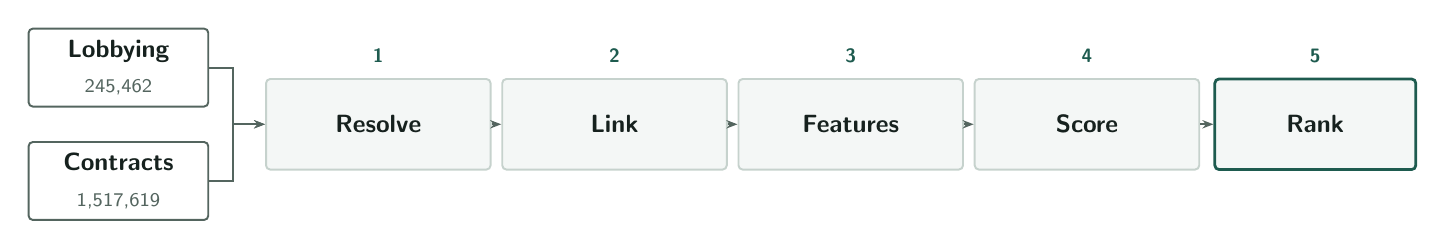
\begin{tikzpicture}[
  font=\sffamily,
  stg/.style={draw=rulec, fill=boxbg, rounded corners=1.5pt, line width=0.7pt,
              text width=2.5cm, align=center, inner sep=5pt, minimum height=1.15cm},
  srcx/.style={draw=slate, rounded corners=1.5pt, line width=0.7pt,
              text width=2.0cm, align=center, inner sep=4pt, minimum height=0.8cm},
  fin/.style={draw=pine, fill=boxbg, rounded corners=1.5pt, line width=1.0pt,
              text width=2.2cm, align=center, inner sep=5pt, minimum height=1.15cm},
  aa/.style={-{Stealth[length=4pt]}, draw=slate, line width=0.7pt},
  nm/.style={font=\sffamily\scriptsize\bfseries, color=pine}]

\node[srcx] (l) at (0,0.72)  {{\hdd Lobbying}\\[1pt]{\sbb 245{,}462}};
\node[srcx] (p) at (0,-0.72) {{\hdd Contracts}\\[1pt]{\sbb 1{,}517{,}619}};
\node[stg] (a) at (3.3,0)  {{\hdd Resolve}};
\node[stg] (b) at (6.3,0)  {{\hdd Link}};
\node[stg] (c) at (9.3,0)  {{\hdd Features}};
\node[stg] (d) at (12.3,0) {{\hdd Score}};
\node[fin] (e) at (15.2,0) {{\hdd Rank}};

\draw[aa] (l.east) -- ++(0.3,0) |- (a.west);
\draw[aa] (p.east) -- ++(0.3,0) |- (a.west);
\draw[aa] (a)--(b); \draw[aa] (b)--(c); \draw[aa] (c)--(d); \draw[aa] (d)--(e);
\node[nm, above=2pt of a] {1}; \node[nm, above=2pt of b] {2};
\node[nm, above=2pt of c] {3}; \node[nm, above=2pt of d] {4};
\node[nm, above=2pt of e] {5};
\end{tikzpicture}
\end{center}

\vspace{0.4em}

\begin{center}
\begin{tabular}{@{}p{1.0cm}p{2.6cm}p{11.6cm}@{}}
\toprule
& \textbf{Step} & \textbf{What happens} \\
\midrule
1 & Resolve   & Many spellings of a company become one entity. A parent and its
                subsidiary stay apart, because merging them would create a case that
                does not exist. \\
2 & Link      & For every contract, we look back for lobbying of the department that
                bought. Lobbying any other department is ignored. \\
3 & Features  & Nine numbers, each between 0 and 1. Larger always means more
                suspicious. \\
4 & Score     & Around 45 small rules are added together. Each rule can only add. \\
5 & Rank      & Sort, then pass the highest to a reporter with the evidence attached. \\
\bottomrule
\end{tabular}
\end{center}

\vspace{0.3em}

The unit is one contract. There are 1{,}497{,}648 of them.

%======================================================================
\section*{The features}

The claim has four parts. The company lobbied that department. The contract followed soon
after. There was no competition. The relationship is unusual. Each feature tests one part.

%---------------------------------------------------------------
\subsection*{Did the lobbying happen, and when?}

\begin{center}\small
\begin{tabular}{@{}p{2.6cm}p{5.6cm}p{6.7cm}@{}}
\toprule
\textbf{Feature} & \textbf{How it is built} & \textbf{What it shows} \\
\midrule
\texttt{f\_recency} &
  $1/(1+\text{gap}/365)$, where the gap is the days from the last registration of that
  department to the award &
  The lobbying was recent enough to still be live. Officials are in post, the budget
  cycle is the same. \\
\texttt{f\_time\_excess} &
  $1-p_{\text{time}}$, where
  $p_{\text{time}} = 1-(1-Q)^{n}$ measured against the national lobbying calendar &
  The closeness is greater than this company's own volume of lobbying would produce
  by chance. \\
\texttt{f\_channel} &
  $\log(1+n)/\log(201)$, where $n$ counts registrations on that channel &
  A sustained campaign rather than a single enquiry. \\
\bottomrule
\end{tabular}
\end{center}

%---------------------------------------------------------------
\subsection*{Was there competition?}

\begin{center}\small
\begin{tabular}{@{}p{2.6cm}p{5.6cm}p{6.7cm}@{}}
\toprule
\textbf{Feature} & \textbf{How it is built} & \textbf{What it shows} \\
\midrule
\texttt{f\_noncomp} &
  1 when \texttt{pro\_award.method} is \texttt{NON}, \texttt{LIMITED} or
  \texttt{ADVANCE}, otherwise 0 &
  Nobody else could bid, so a person chose the supplier. This is the condition that
  makes influence possible. \\
\texttt{f\_nc\_rarity} &
  $1-\dfrac{k+5(0.226)}{n+5}$, using that department's own record &
  An exception was made. A department that always awards this way tells us nothing;
  one that rarely does tells us a great deal. \\
\texttt{f\_tender\_short} &
  $1-$ the share of all tenders whose window was this short &
  The process left little room for anyone else to respond. \\
\bottomrule
\end{tabular}
\end{center}

%---------------------------------------------------------------
\subsection*{Is the relationship unusual?}

\begin{center}\small
\begin{tabular}{@{}p{2.6cm}p{5.6cm}p{6.7cm}@{}}
\toprule
\textbf{Feature} & \textbf{How it is built} & \textbf{What it shows} \\
\midrule
\texttt{f\_dominance} &
  $1-P(X \ge N)$ with $X \sim \mathrm{Bin}(n_{\text{dept}},\, 1/m_{\text{suppliers}})$ &
  One supplier holds far more of the department's work than an even split would give.
  A relationship rather than a market. \\
\texttt{f\_dep\_share} &
  Contracts with this department divided by the supplier's total &
  The supplier depends on this department, which creates an incentive to protect the
  relationship. \\
\bottomrule
\end{tabular}
\end{center}

%---------------------------------------------------------------
\subsection*{Would a reporter care?}

\begin{center}\small
\begin{tabular}{@{}p{2.6cm}p{5.6cm}p{6.7cm}@{}}
\toprule
\textbf{Feature} & \textbf{How it is built} & \textbf{What it shows} \\
\midrule
\texttt{f\_prominence} &
  $\log(1+\text{total awards})/\log(20001)$ &
  A large and recognisable organisation. Newsworthiness rather than anomaly. \\
\bottomrule
\end{tabular}
\end{center}

%======================================================================
\section*{Where the features come from}

\begin{center}\small
\begin{tabular}{@{}p{5.4cm}p{1.4cm}p{7.6cm}@{}}
\toprule
\textbf{Source} & \textbf{Count} & \textbf{Features} \\
\midrule
A column read straight from the data & 1 &
  \texttt{f\_noncomp} \\
A probability against a reference population & 4 &
  \texttt{f\_time\_excess}, \texttt{f\_nc\_rarity}, \texttt{f\_tender\_short},
  \texttt{f\_dominance} \\
A count rolled up per company or department & 3 &
  \texttt{f\_channel}, \texttt{f\_dep\_share}, \texttt{f\_prominence} \\
Date arithmetic on the link itself & 1 &
  \texttt{f\_recency} \\
\bottomrule
\end{tabular}
\end{center}

The three rolled up features hold the same value for every contract a company has. They
can separate one company from another, but not one contract from another.

%======================================================================
\section*{The funnel}

\begin{center}\small
\begin{tabular}{@{}lrr@{}}
\toprule
\textbf{Stage} & \textbf{Count} & \textbf{Share} \\
\midrule
Contracts scored                        & 1{,}497{,}648 & 100\% \\
With lobbying of the buying department  &   136{,}583 &  9.1\% \\
Awarded without competition             &   304{,}516 & 20.3\% \\
Both conditions together                &    31{,}168 &  2.1\% \\
Both, and within 90 days                &    11{,}406 &  0.8\% \\
\bottomrule
\end{tabular}
\end{center}

\end{document}
